\chapter{Dyskusja rezultatów}

\section{Przykładowe wyniki}
\subsection{Wynik dla przykładu ze wstępu}
Wracając do dziennika zdarzeń przedstawionego w sekcji \ref{sec:event_logs}, a dla którego stworzono przykładowy model i obliczono metryki w sekcji \ref{sec:alignment-calculation}. 
\begin{figure}[!ht]
	\centering{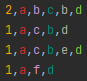
\includegraphics{datasets/v4a6c5l5.png}}
	\caption{\label{fig:flow_chart}Warianty procesu}
\end{figure}

Przy odkrywaniu modelu dla tego wariantu użyto następujących wag poszczególnych metryk: odwzorowanie = 18, złożoność = 2, generalizacja = 2, precyzja = 12, prostota = 2. Model dla tego dziennika zdarzeń znaleziony przy pomocy algorytmu to:
\begin{center}
	\{a\}xor(seq(opt(\{b\})\{c\}\{b\}opt(\{e\}))\{f\})\{d\}
\end{center}
oraz graficznie:

\begin{figure}[!ht]
	\centering{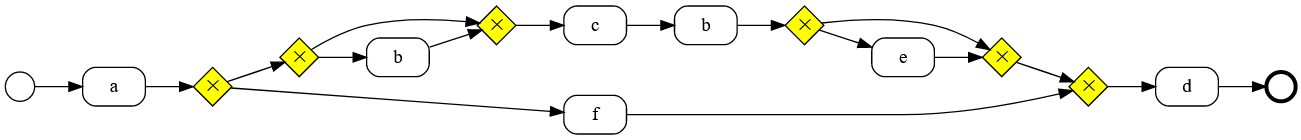
\includegraphics[scale=0.37]{examples/v4a6c5l5.csv_run-686_21_3_21_184242_35664_645567/graphviz.png}}
	\caption{\label{fig:flow_chart}Znaleziony model}
\end{figure}

Do znalezienia modelu potrzebne były 522 generacje, podczas których przeszukano 97771 unikalnych osobników. Zajęło to 1052.8 sekund, używając 4 wątków procesora. Natomiast, metryki mają następujące wartości: 

 \begin{center}
  \begin{tabular}{l}
	Średnia ważona: 0.9550 \\
	Odwzorowanie: 1.0 \\
	Złożoność: 1.0 \\
	Generalizacja: 0.3426 \\
	Precyzja: 0.9875 \\
	Prostota: 0.9231
  \end{tabular}
 \end{center}

Dla porównania poszczególne metryki obliczone w sekcji \ref{sec:alignment-calculation} wynosiły odwzorowanie = 0.9243, złożoność = 0.9706, generalizacja = 0.3997, precyzja = 0.9465, prostota = 0.8333, a średnia ważona używając przyjętych wag, wyniosłaby 0.9001. Używając algorytmu ewolucyjnego, otrzymano więc znacznie lepszy model.

Poniżej zaprezentowano również wykres, na który zaprezentowano zmianę wartości metryk w kolejnych generacjach. Jest on generowany podczas działania algorytmu i kończy się w momencie przerwania działania algorytmu lub po określonej ilości iteracji, a nie znalezienia rozwiązania, gdyż przy algorytmach ewolucyjnych nie można być pewnym, czy znaleziono najlepsze rozwiązanie.
\begin{figure}[!ht]
	\centering{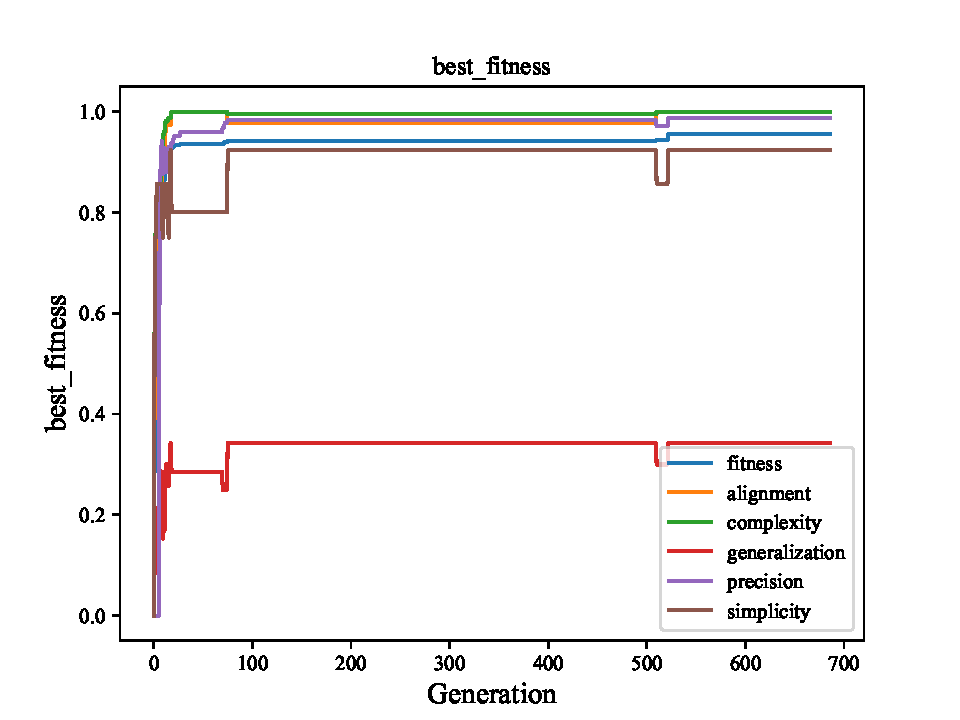
\includegraphics[scale=0.85]{examples/v4a6c5l5.csv_run-686_21_3_21_184242_35664_645567/best_fitness.pdf}}
	\caption{\label{fig:flow_chart}Przebieg ewolucji}
\end{figure}
\clearpage

\subsection{Inne przykłady działania}

Przykładowe dziennik zdarzeń wzięto z \cite{pm-book}. Część z nich została wygenerowania sztucznie, a część zawiera realne dane. Następnie przerobiono je na warianty procesu. 

\subsubsection{Przykład \#1}
Prosty sztucznie wygenerowany przykład. Zawiera 6 unikalnych aktywności, 13 przypadków, 6 wariantów, z których najdłuższy ma 12 zdarzeń. 
\begin{figure}[H]
	\centering{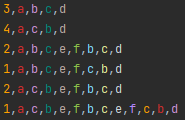
\includegraphics[scale=0.8]{datasets/v6a6c13l12.png}}
	\caption{\label{fig:flow_chart}Warianty procesu}
\end{figure}

Przy odkrywaniu modelu dla tego wariantu użyto następujących wag poszczególnych metryk: odwzorowanie = 8, złożoność = 2, generalizacja = 2, precyzja = 2, prostota = 2. Model dla tego dziennika zdarzeń znaleziony przy pomocy algorytmu to:
\begin{center}
	\{a\}and(\{b\}\{c\})lo4(\{e\}\{f\}and(\{b\}\{c\}))\{d\}
\end{center}
oraz graficznie:

\begin{figure}[H]
	\centering{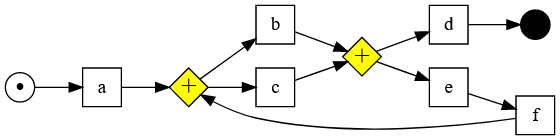
\includegraphics[scale=0.37]{examples/v6a6c13l12.csv_run-84_21_3_2_222502/graphviz.png}}
	\caption{\label{fig:flow_chart}Znaleziony model}
\end{figure}

Do znalezienia modelu potrzebne były 83 generacje, podczas których przeszukano 20338 unikalnych osobników. Zajęło to 321.5 sekund, używając 4 wątków procesora. Natomiast, metryki mają następujące wartości: 

 \begin{center}
  \begin{tabular}{l}
	Średnia ważona: 0.9606 \\
	Odwzorowanie: 1.0 \\
	Złożoność: 1.0 \\
	Generalizacja: 0.7019 \\
	Precyzja: 0.9830 \\
	Prostota: 1.0
  \end{tabular}
 \end{center}
 
\begin{figure}[H]
	\centering{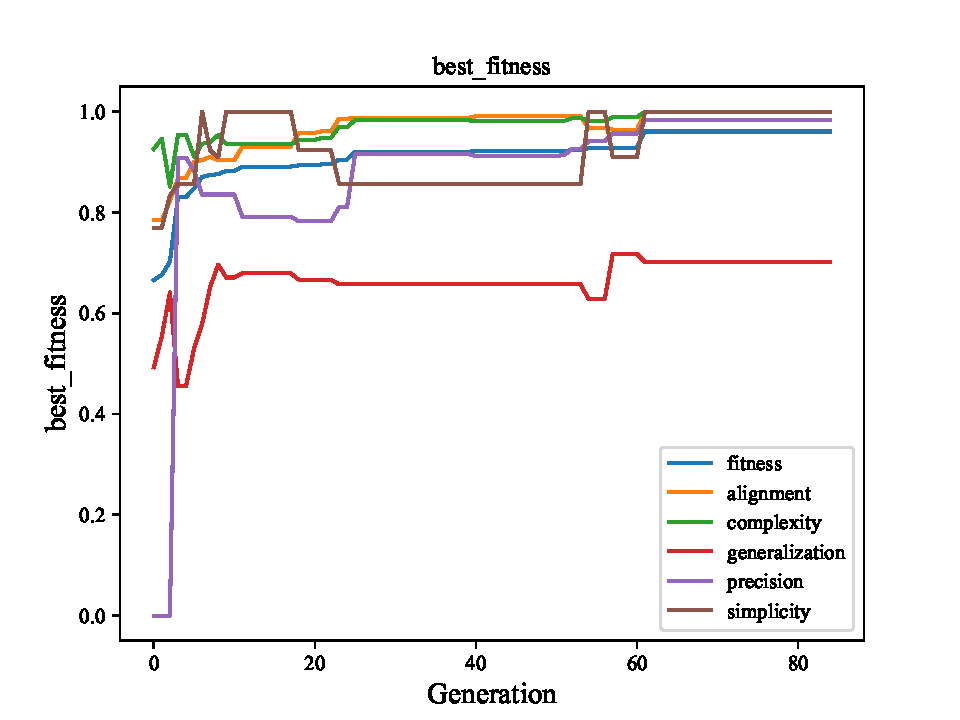
\includegraphics[scale=0.83]{examples/v6a6c13l12.csv_run-84_21_3_2_222502/best_fitness.pdf}}
	\caption{\label{fig:flow_chart}Przebieg ewolucji}
\end{figure}

\subsubsection{Przykład \#2}
Kolejny prosty sztucznie wygenerowany przykład. Zawiera 5 unikalnych aktywności, 40 przypadków, 8 wariantów, z których najdłuższy ma 5 zdarzeń. 

\begin{figure}[H]
	\centering{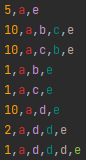
\includegraphics[scale=0.8]{datasets/v8a5c40l5.png}}
	\caption{\label{fig:flow_chart}Warianty procesu}
\end{figure}

Przy odkrywaniu modelu dla tego wariantu użyto następujących wag poszczególnych metryk: odwzorowanie = 8, złożoność = 2, generalizacja = 2, precyzja = 2, prostota = 2. Model dla tego dziennika zdarzeń znaleziony przy pomocy algorytmu to:
\begin{center}
	\{a\}lo2(\{d\})opt(\{b\}\{c\})\{e\}
\end{center}
oraz graficznie:

\begin{figure}[H]
	\centering{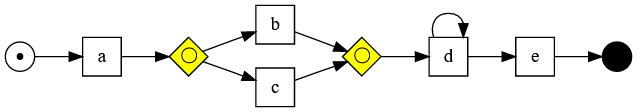
\includegraphics[scale=0.37]{examples/v8a5c40l5.csv_run-24_21_3_6_211037_47336_515221/graphviz.png}}
	\caption{\label{fig:flow_chart}Znaleziony model}
\end{figure}

Do znalezienia modelu potrzebne było 11 generacji, podczas których przeszukano 3636 unikalnych osobników. Zajęło to 75.2 sekund, używając 4 wątków procesora. Natomiast, metryki mają następujące wartości: 

 \begin{center}
  \begin{tabular}{l}
	Średnia ważona: 0.9722 \\
	Odwzorowanie: 1.0 \\
	Złożoność: 1.0 \\
	Generalizacja: 0.7940 \\
	Precyzja: 0.9834 \\
	Prostota: 1.0
  \end{tabular}
 \end{center}
 
\begin{figure}[H]
	\centering{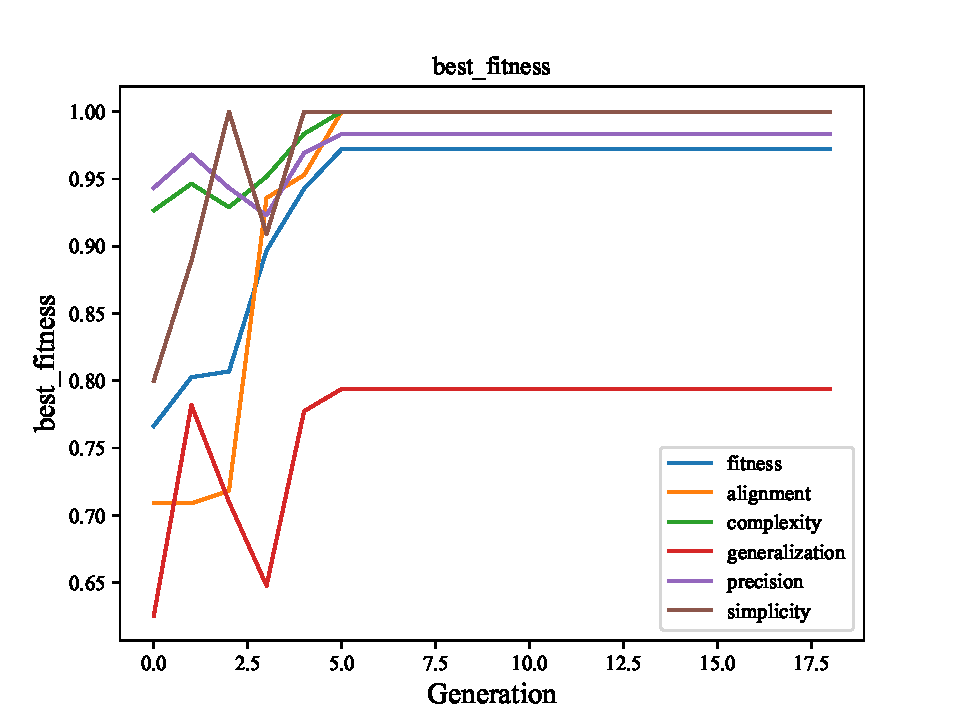
\includegraphics[scale=0.83]{examples/v8a5c40l5.csv_run-24_21_3_6_211037_47336_515221/best_fitness.pdf}}
	\caption{\label{fig:flow_chart}Przebieg ewolucji}
\end{figure}

\subsubsection{Przykład \#Obsługa roszczeń w firmie ubezpieczeniowej}
Dziennik danych zawiera dane opisujące obsługa roszczeń w firmie ubezpieczeniowej. Proces może być obsługiwany przez dwie różne działy w Brisbane i Sydney. Możliwe jest połączenie danych dla tych działów, ale nie zrobiono tego, żeby utrudnić odkrywanie modelu.
Przykład składa się z 11 unikalnych aktywności, 3512 przypadków, 12 wariantów, z których najdłuższy ma 9 zdarzeń. 

\begin{figure}[H]
	\centering{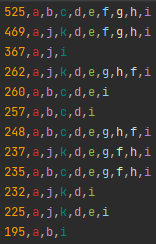
\includegraphics[scale=0.8]{datasets/v12a11c3512l9.png}}
	\caption{\label{fig:flow_chart}Warianty procesu}
\end{figure}

Przy odkrywaniu modelu dla tego wariantu użyto następujących wag poszczególnych metryk: odwzorowanie = 8, złożoność = 2, generalizacja = 2, precyzja = 2, prostota = 2. Model dla tego dziennika zdarzeń znaleziony przy pomocy algorytmu to:
\begin{center}
	\{a\}opt(xor(\{j\}\{b\})\{k\})opt(opt(\{d\}\{e\})\{c\})opt(and(\{f\}\{h\}\{g\}))\{i\}
\end{center}
oraz graficznie:

\begin{figure}[H]
	\centering{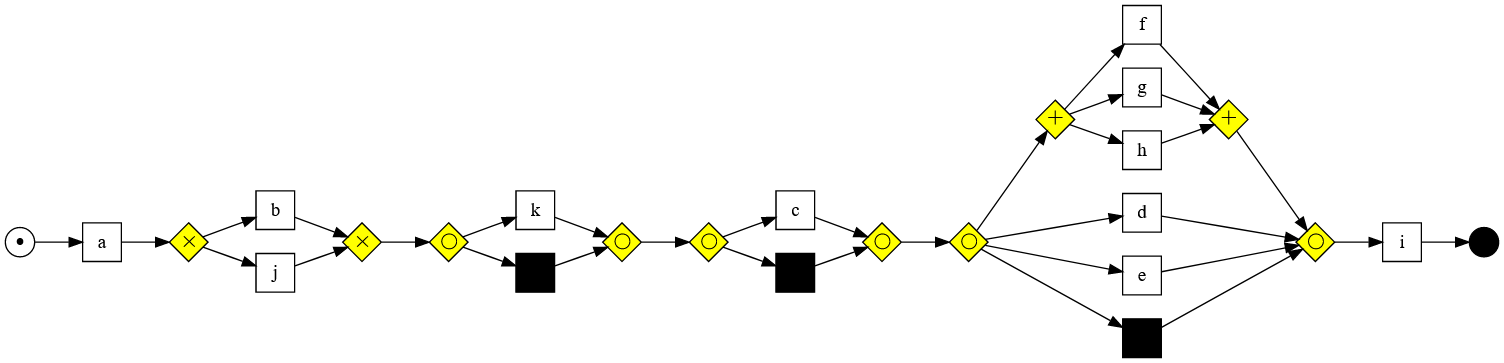
\includegraphics[scale=0.3]{examples/v12a11c3512l9.csv_run-10231_21_3_1_042344_29708_523416/graphviz.png}}
	\caption{\label{fig:flow_chart}Znaleziony model}
\end{figure}

Do znalezienia modelu potrzebne było 4110 generacji. Zajęło to 17157.7 sekund, używając 4 wątków procesora. Natomiast, metryki mają następujące wartości: 

 \begin{center}
  \begin{tabular}{l}
	Średnia ważona: 0.9748 \\
	Odwzorowanie: 1.0 \\
	Złożoność: 1.0 \\
	Generalizacja: 0.9782 \\
	Precyzja: 0.8204 \\
	Prostota: 1.0
  \end{tabular}
 \end{center}
 
\begin{figure}[H]
	\centering{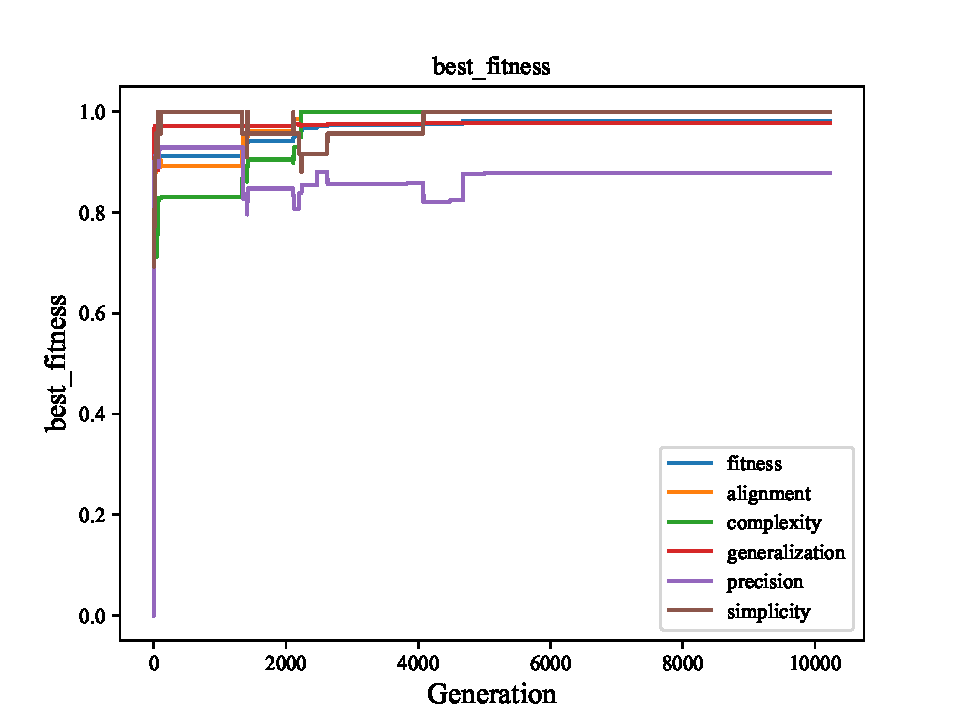
\includegraphics[scale=0.73]{examples/v12a11c3512l9.csv_run-10231_21_3_1_042344_29708_523416/best_fitness.pdf}}
	\caption{\label{fig:flow_chart}Przebieg ewolucji}
\end{figure}

\subsubsection{Przykład \#Naprawa telefonu}
Dziennik zdarzeń zawiera dane dotyczące procesu naprawy telefonu.
Przykład składa się z 7 unikalnych aktywności, 1000 przypadków, 45 wariantów, z których najdłuższy ma 14 zdarzeń. 

\begin{figure}[H]
	\centering{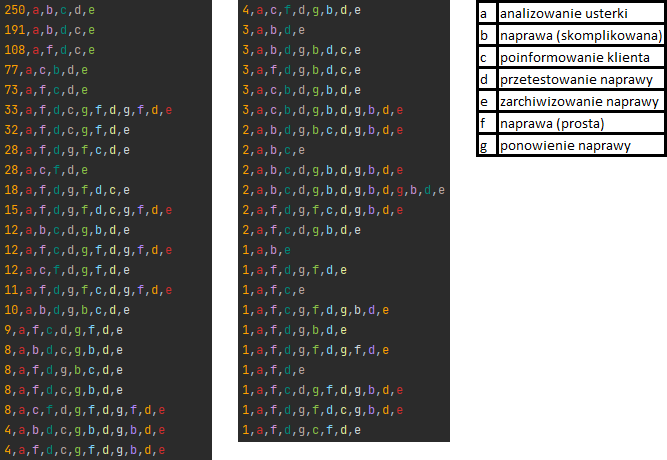
\includegraphics[scale=0.8]{datasets/v45a7c1000l14.png}}
	\caption{\label{fig:flow_chart}Warianty procesu}
\end{figure}

Przy odkrywaniu modelu dla tego wariantu użyto następujących wag poszczególnych metryk: odwzorowanie = 8, złożoność = 2, generalizacja = 2, precyzja = 4, prostota = 1. Model dla tego dziennika zdarzeń znaleziony przy pomocy algorytmu to:
\begin{center}
	\{a\}xor(\{f\}\{b\})and(\{d\}opt(\{c\}))lo3(\{g\}xor(\{f\}\{b\})and(\{d\}opt(\{c\})))\{e\}
\end{center}
oraz graficznie:

\begin{figure}[H]
	\centering{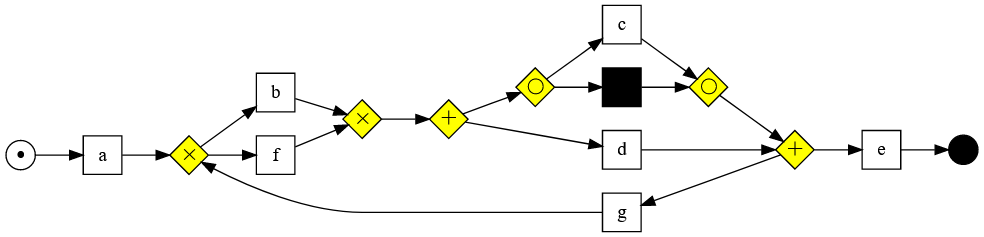
\includegraphics[scale=0.37]{examples/v45a7c1000l14.csv_run-1366_21_3_6_143708_2144_563150/graphviz.png}}
	\caption{\label{fig:flow_chart}Znaleziony model}
\end{figure}

Do znalezienia modelu potrzebne było 436 generacji. Zajęło to 4675.0 sekund, używając 4 wątków procesora. Natomiast, metryki mają następujące wartości: 

 \begin{center}
  \begin{tabular}{l}
	Średnia ważona: 0.9859 \\
	Odwzorowanie: 0.9896 \\
	Złożoność: 0.9891 \\
	Generalizacja: 0.9614 \\
	Precyzja: 0.9859 \\
	Prostota: 1.0
  \end{tabular}
 \end{center}
 
\begin{figure}[H]
	\centering{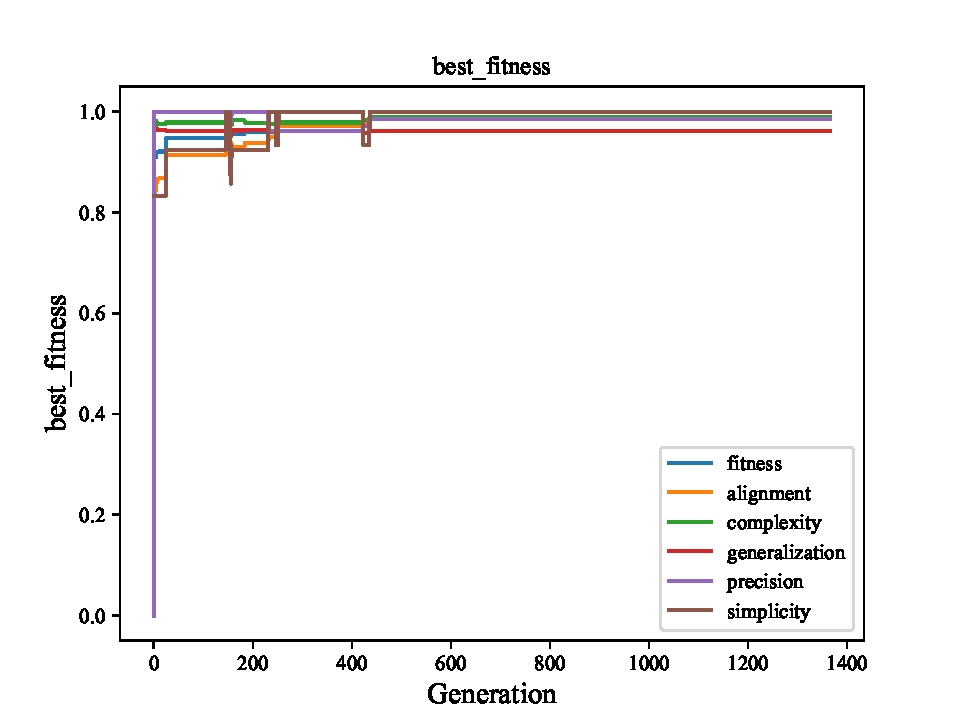
\includegraphics[scale=0.72]{examples/v45a7c1000l14.csv_run-1366_21_3_6_143708_2144_563150/best_fitness.pdf}}
	\caption{\label{fig:flow_chart}Przebieg ewolucji}
\end{figure}

\subsubsection{Przykład \#Obsługa wniosku o odszkodowanie}
\label{sec:example5}
Dziennik zdarzeń zawiera dane obsługi wniosku o odszkodowanie.
Przykład składa się z 8 unikalnych aktywności, 1391 przypadków, 21 wariantów, z których najdłuższy ma 17 zdarzeń. 
\begin{figure}[!ht]
	\centering{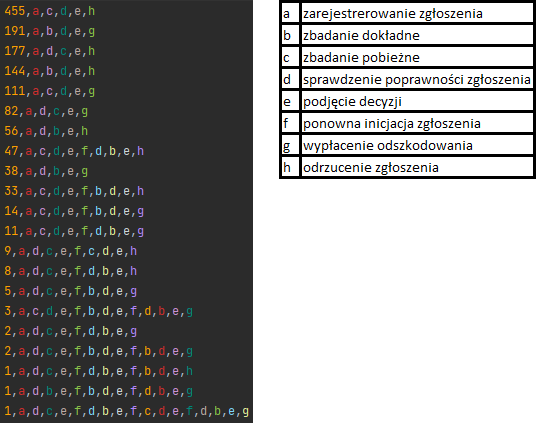
\includegraphics[scale=0.8]{datasets/v21a81391l17.png}}
	\caption{\label{fig:flow_chart}Warianty procesu}
\end{figure}

Przy odkrywaniu modelu dla tego wariantu użyto następujących wag poszczególnych metryk: odwzorowanie = 8, złożoność = 2, generalizacja = 2, precyzja = 2, prostota = 2. Model dla tego dziennika zdarzeń znaleziony przy pomocy algorytmu to:
\begin{center}
	\{a\}lo1(\{f\}and(\{d\}xor(\{b\}\{c\}))\{e\})xor(\{g\}\{h\})
\end{center}
oraz graficznie:

\begin{figure}[H]
	\centering{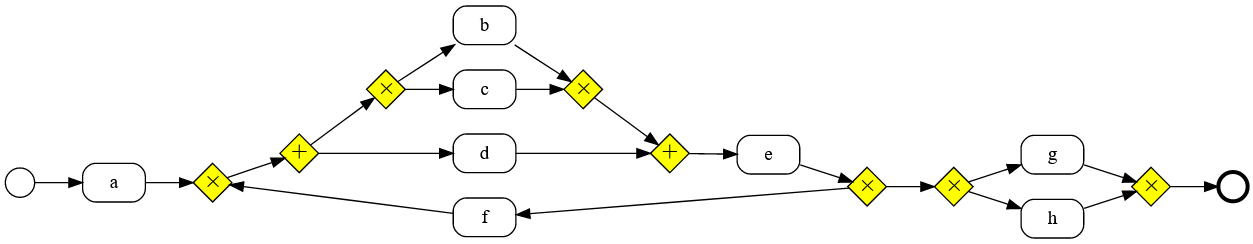
\includegraphics[scale=0.37]{examples/v21a81391l17.csv_run-15614_21_3_1_225455/graphviz.png}}
	\caption{\label{fig:flow_chart}Znaleziony model}
\end{figure}

Do znalezienia modelu potrzebne było 2270 generacji, podczas których przeszukano 319963 unikalnych osobników. Zajęło to 15123.3 sekund, używając 4 wątków procesora. Natomiast, metryki mają następujące wartości: 

 \begin{center}
  \begin{tabular}{l}
	Średnia ważona: 0.9940 \\
	Odwzorowanie: 1.0 \\
	Złożoność: 1.0 \\
	Generalizacja: 0.9624 \\
	Precyzja: 0.9899 \\
	Prostota: 1.0
  \end{tabular}
 \end{center}
 
\begin{figure}[H]
	\centering{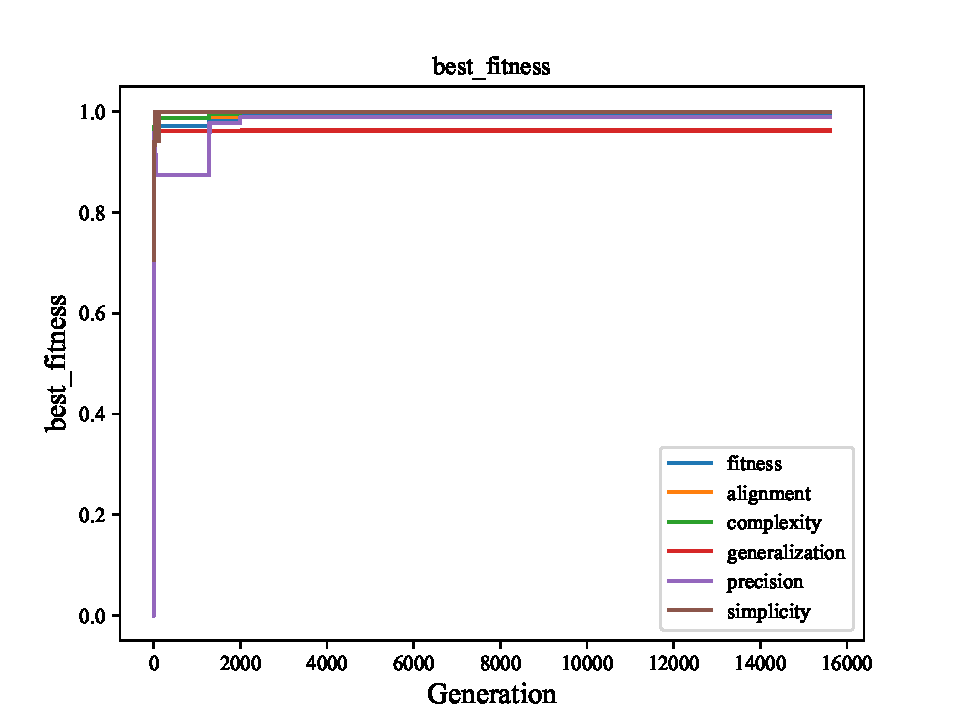
\includegraphics[scale=0.83]{examples/v21a81391l17.csv_run-15614_21_3_1_225455/best_fitness.pdf}}
	\caption{\label{fig:flow_chart}Przebieg ewolucji}
\end{figure}

\section{Wyniki w zależności od przyjętych wag poszczególnych metryk}

\subsection{Brak poszczególnych metryk}
Odwzorowanie jest kluczowe, gdyż jest jedyną metryką, która sprawdza zgodność modelu z dziennikiem zdarzeń i bez tej metryki model byłby pozbawiony wartości. Pozostałe metryki wpływają na jego jakość. Warto więc sprawdzić jak ich brak wpłynąłby na jego odkryty model.

\subsubsection{Poprawny model}
Wpływ brak poszczególny metryk sprawdzony dla podzbioru dziennika zdarzeń z sekcji \ref{sec:example5} uproszczonego poprzez pozbawienie go pętli. Dla porównania przedstawiono poprawny model, odkryty używając wszystkich metryk.
Składa się on z 7 unikalnych aktywności, 1254 przypadków, 8 wariantów, które mają po 5 zdarzeń. 
\begin{figure}[!ht]
	\centering{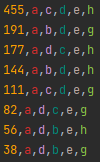
\includegraphics[scale=0.8]{datasets/v8a7c1254l5.png}}
	\caption{\label{fig:flow_chart}Warianty procesu}
\end{figure}

Przy odkrywaniu modelu dla tego wariantu użyto następujących wag poszczególnych metryk: odwzorowanie = 8, złożoność = 2, generalizacja = 2, precyzja = 4, prostota = 2. Model dla tego dziennika zdarzeń znaleziony przy pomocy algorytmu to:
\begin{center}
	\{a\}and(xor(\{c\}\{b\})\{d\})\{e\}xor(\{h\}\{g\})
\end{center}
oraz graficznie:

\begin{figure}[!ht]
	\centering{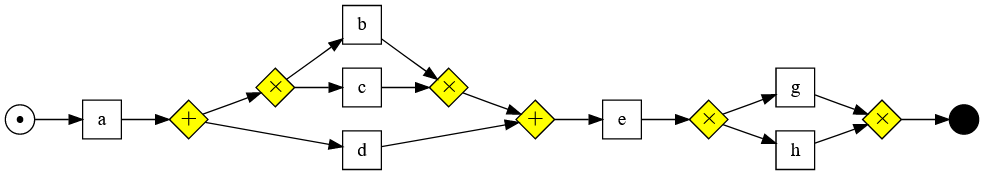
\includegraphics[scale=0.37]{examples/v8a7c1254l5.csv_run-303_21_3_5_003759/graphviz.png}}
	\caption{\label{fig:flow_chart}Znaleziony model}
\end{figure}

Do znalezienia modelu potrzebne były 233 generacje, podczas których przeszukano 41537 unikalnych osobników. Zajęło to 504.2 sekund, używając 4 wątków procesora. Natomiast, metryki mają następujące wartości: 

 \begin{center}
  \begin{tabular}{l}
	Średnia ważona: 0.9960 \\
	Odwzorowanie: 1.0 \\
	Złożoność: 1.0 \\
	Generalizacja: 0.9641 \\
	Precyzja: 1.0 \\
	Prostota: 1.0
  \end{tabular}
 \end{center}

\subsubsection{Brak precyzji}
Te same metryki jednak precyzja = 0.
Model graficznie:
\begin{figure}[!ht]
	\centering{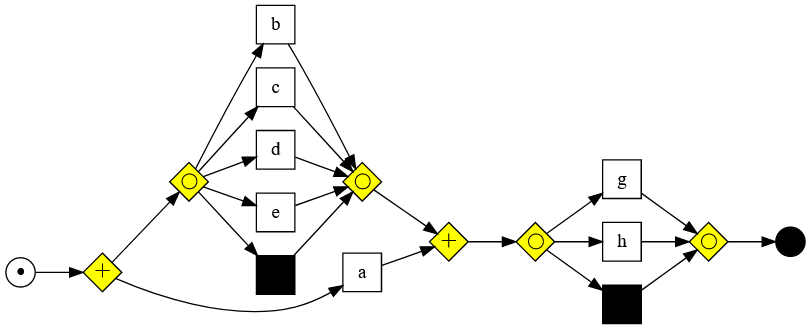
\includegraphics[scale=0.37]{examples/v8a7c1254l5.csv_21_4_13_211038_8672_3/graphviz.png}}
	\caption{\label{fig:flow_chart}Znaleziony model}
\end{figure}

 \begin{center}
  \begin{tabular}{l}
	Średnia ważona: 0.9289 \\
	Odwzorowanie: 1.0 \\
	Złożoność: 1.0 \\
	Generalizacja: 0.9641 \\
	Precyzja: 0.6982 \\
	Prostota: 1.0
  \end{tabular}
 \end{center}
 
\subsubsection{Brak prostoty i generalizacji}
Te same metryki jednak prostota = 0 i generalizacja = 0.
Model graficznie:
\begin{figure}[!ht]
	\centering{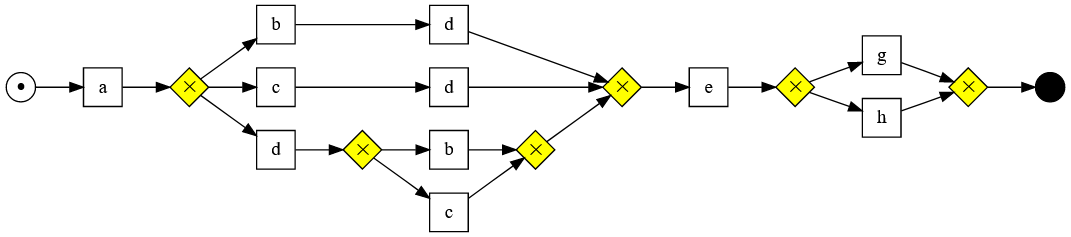
\includegraphics[scale=0.37]{no-generalization-and-simplicity.png}}
	\caption{\label{fig:flow_chart}Znaleziony model}
\end{figure}

 \begin{center}
  \begin{tabular}{l}
	Średnia ważona: 0.9697 \\
	Odwzorowanie: 1.0 \\
	Złożoność: 1.0 \\
	Generalizacja: 0.9498 \\
	Precyzja: 1.0 \\
	Prostota: 0.7778
  \end{tabular}
 \end{center}

\subsection{Wpływ złożoności na wynik}

\section{Wnioski}
Najbardziej na działanie wpływa

Coś odnośnie metryk
